\section{Recurrent neural network architecture}

%%%%%%%%%%%%%%%%%%%%%%%%%%%%%
\begin{figure*}[htb]
\centering
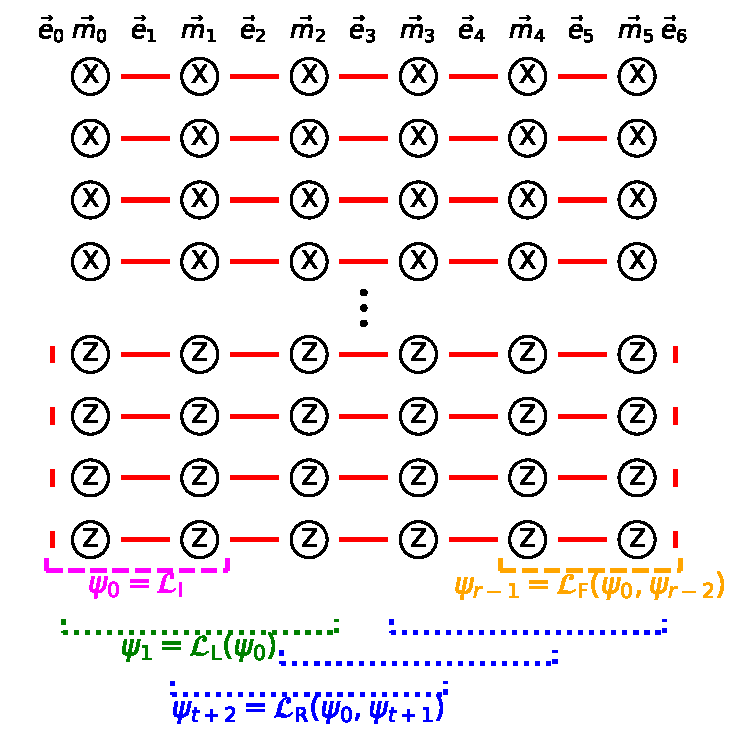
\includegraphics[width=0.9\textwidth]{RCNN_layer_progression_d3_r6.pdf}
\ccaption
{Layer progression in the recurrent NN architecture}
{
Illustrated is an example for a memory experiment over the logical $Z_L$ observable in an arbitrary distance-$d$ surface code with $r=6$ rounds. Each column of circles marks a different stabilizer measurement round, with the circles corresponding to the readings from the $X$ or $Z$ measure qubits, $\vec{m}_t$ for $0\leq t \leq r-1$. The horizontal red lines mark detector events that check for the consistency of measure qubit readings, $\vec{e}_t$ for $1 \leq t \leq r-1$, and the vertical red lines next to the $Z$ measure qubit readings mark the unique detector events associated with these readings at the beginning, $\vec{e}_0$, and end of the memory experiment, $\vec{e}_{r}$.
Each bracket at the bottom corresponds to a different pass in the recurrent architecture, with the extent of the brackets demarcating the measure qubit readings and detector events that are used as input features.
The initialization layer, $\mathcal{L}_I$ (magenta), provides an initial error state $\psi_0$ from $\vec{m}_0$, $\vec{m}_1$, $\vec{e}_0$, and $\vec{e}_1$.
The lead-in layer, $\mathcal{L}_L$ (green), updates the error state to $\psi_1$ using the first available triplet stabilizer state parametrization from $\vec{m}_{0 \text{---} 2}$, $\vec{e}_1$ and $\vec{e}_2$, and the state $\psi_0$.
The recurrent layer, $\mathcal{L}_R$ (blue), then strides through the rest of rounds one by one; to obtain each error state update $\psi_{t+2}$ ($t\geq0$), this layer uses the triplet stabilizer state parametrization from $\vec{m}_{(t+1) \text{---} (t+3)}$, $\vec{e}_{t+2}$ and $\vec{e}_{t+3}$, the previous error state $\psi_{t+1}$, and the initial error state $\psi_{0}$.
At the end, the finalization layer, $\mathcal{L}_F$ (orange), provides the final error state prediction $\psi_{r-1}$ upon receiving $\vec{m}_{r-2}$ and $\vec{m}_{r-1}$, $\vec{e}_{r-1}$ and $\vec{e}_r$, and the last known error state $\psi_{r-2}$ and the initial error state $\psi_{0}$.
}
\label{fig:RCNN-layer-prog}
\end{figure*}
%%%%%%%%%%%%%%%%%%%%%%%%%%%%%
